\documentclass{article}
\usepackage{graphicx}
\usepackage[margin=2.5cm]{geometry}
\usepackage{listings}
\lstset{language=Python}
\usepackage{hyperref}
\usepackage{minted}
\usepackage{amsmath}
\usepackage{tikz, pgfplots}
\usetikzlibrary{positioning}
\usepackage{parskip}
\usepackage{adjustbox}
\usepackage{amssymb}
\usepackage{subcaption}

\title{LA Project}
\author{Nijesh Raghava}
\date{June 2023}

\begin{document}

\maketitle

\section{Methodology}
\subsection{Wavelet Transformation}
\setlength{\parindent}{1cm}
Haar wavelet compression is an efficient way to perform both lossless and lossy image compression. It relies on averaging and differentiating values in an image matrix to produce Wavelet Transform.

\begin{center}
  \large\textbf{Averaging and Differentiating}
\end{center}

\setlength{\parindent}{1cm}
To understand how the technique works, let us start with an example. As the computer system deals the image as a matrix or an array of discrete values known as ‘‘pixels’’ or ‘‘picture elements,’’ these discrete values range from 0 (black) to some positive number values 255 (white). For computing the Haar wavelet of an image, we must convert an image to a discrete matrix as Haar wavelet transform cannot deal with continuous data, and discrete matrix of an image can be achieved using MATLAB (a programming tool). In this paper, we considered only an 8x8 image block for processing but note that the same technique is applied to the whole image to calculate the HWT of the image.

\begin{equation*}
    P = \begin{bmatrix}
        576 & 704 & 1152 & 1280 & 1344 & 1472 & 1536 & 1536 \\
        704 & 640 & 1156 & 1088 & 1344 & 1408 & 1536 & 1600 \\
        768 & 832 & 1216 & 1472 & 1472 & 1536 & 1600 & 1600 \\
        832 & 832 & 960 & 1344 & 1536 & 1536 & 1600 & 1536 \\
        832 & 832 & 960 & 1216 & 1536 & 1600 & 1536 & 1536 \\
        960 & 896 & 896 & 1088 & 1600 & 1600 & 1600 & 1536 \\
        768 & 768 & 832 & 832 & 1280 & 1472 & 1600 & 1600 \\
        448 & 768 & 704 & 640 & 280 & 1408 & 1600 & 1600 \\
    \end{bmatrix}_{8\times8}    
\end{equation*}

\setlength{\parindent}{1cm}
To convert matrix ‘‘P’’ to wavelet transform, first we will find the average and difference of each row and column of the matrix, as these are required for computing Haar wavelet transform of an image. The following steps were applied to obtain a transformed matrix:
\begin{itemize}
    \item Deal each vector (row) of the matrix as a string. 
    \item Now, group all of the columns in pairs
    \item We replace the first 4 columns of row with the average of these pairs and replace the last 4 columns with ½ of the difference of these pairs.  
    \item We repeat the process until desired level of compression or decomposition is reached and is repeated on all the rows of the matrix
\end{itemize}

\setlength{\parindent}{1cm}
Initially the first row of P
\begin{equation*}
    P_1  = \begin{bmatrix}
        576 & 704 & 1152 & 1280 & 1344 & 1472 & 1536 & 1536 \\
    \end{bmatrix}
\end{equation*}

\setlength{\parindent}{1cm}
Averaging and differentiating the first row of P results in :
\begin{equation*}
    P_1 = \begin{bmatrix}
        640 & 1216 & 1408 & 1536 & -64 & -64 & -64 & 0 \\
    \end{bmatrix}
\end{equation*}

\setlength{\parindent}{1cm}
Averaging and differentiating the first row of P again results in :
\begin{equation*}
    P_1 = \begin{bmatrix}
        928 & 1472 & -288 & -64 & -64 & -64 & -64 & 0 \\
    \end{bmatrix}
\end{equation*}

\setlength{\parindent}{1cm}
and averaging and differentiating the first row of P for the third time we get :
\begin{equation*}
    P_1 = \begin{bmatrix}
        1200 & -272 & -288 & -64 & -64 & -64 & -64 & 0 \\
    \end{bmatrix}
\end{equation*}

\setlength{\parindent}{1cm}
As the averaging and differentiating is a reversible process, we can work back from any row to the previous row in the table and hence to the first row using appropriate addition and subtraction techniques. Here, in the whole transformation process, we lost nothing. After completing the transformation process on rows, we will repeat the same transformation process on the columns to achieve high compression. This can be achieved by applying transpose to the row transformed matrix. This gives another matrix "T" with an 8x8 dimension, called Haar wavelet transforms of the table "P" as shown. 

\begin{equation*}
T = \begin{bmatrix}
    1212 & -306 & -146 & -54 & -24 & -68 & -40 & 4 \\
    30 & 36 & -90 & -2 & 8 & -20 & 8 & -4 \\
    -50 & -10 & -20 & -24 & 0 & 72 & -16 & -16 \\
    82 & 38 & -24 & 68 & 48 & -64 & 32 & 8 \\
    8 & 8 & -32 & 16 & -48 & -48 & -16 & 16 \\
    20 & 20 & -56 & -16 & -16 & 32 & -16 & -16 \\
    -8 & 8 & -48 & 0 & -16 & -16 & -16 & -16 \\
    44 & 36 & 0 & 8 & 80 & -16 & -16 & 0 \\
\end{bmatrix}
\end{equation*}

\setlength{\parindent}{1cm}
The matrix T has an overall average value at the top and 63 detail elements. These detail elements are used to capture the high frequency components or details of the original data.The matrix T is called the wavelet-transformed matrix of the matrix P. A matrix with a high proportion of zeros is called a sparse matrix. Corresponding wavelet-transformed matrices of many images are sparser than the original image matrices and that is why it is easier and efficient to transmit and store a matrix that is more sparse than an ordinary matrix of the same size. 

\setlength{\parindent}{1cm}
So, if we transmit the wavelet-transformation matrix, which is essentially the compressed version of the image, we can easily reconstruct the original image by applying some addition and subtraction techniques. We can also decrease the size or details of the image to be reconstructed to a significant level by using a process called thresholding.

\setlength{\parindent}{1cm}
Thresholding involves setting a non-negative threshold value that helps us reduce the amount of information in the detail elements, thereby achieving compression. After obtaining the detail elements, any absolute value of the detail value that falls below this threshold is considered insignificant or negligible and can be set to zero. 

\setlength{\parindent}{1cm}
Let us define the threshold value of as 20, then a matrix D is obtained after thresholding T 

\begin{equation*}
D =
\begin{bmatrix}
1212 & -306 & -146 & -54 & -24 & -68 & -40 & 0 \\
30 & 36 & -90 & 0 & 0 & 0 & 0 & 0 \\
-50 & 0 & 0 & -24 & 0 & 72 & 0 & 0 \\
82 & 38 & -24 & 68 & 48 & -64 & 32 & 0 \\
0 & 0 & -32 & 0 & -48 & -48 & 0 & 0 \\
0 & 0 & -56 & 0 & 0 & 32 & 0 & 0 \\
0 & 0 & -48 & 0 & 0 & 0 & 0 & 0 \\
44 & 36 & 0 & 8 & 80 & 0 & 0 & 0 \\
\end{bmatrix}
\end{equation*}

\setlength{\parindent}{1cm}
After applying the inverse transformation on the matrix D we get the another matrix that has nearly similar values as the matrix P(of course this depends on selecting the threshold value) but when the image is reconstructed from the new matrix its size going to be significantly less than the original image at the cost of quality of the image. The quality of the new image will be quite less than the quality of the original image because we have ignored the detail values that are less than 20. Here is the new matrix that is obtained after reconstructing. 


\begin{equation*}
R = \begin{bmatrix}
582 & 726 & 1146 & 1234 & 1344 & 1424 & 1540 & 1540 \\
742 & 694 & 1178 & 1074 & 1344 & 1424 & 1540 & 1540 \\
706 & 754 & 1206 & 1422 & 1492 & 1572 & 1592 & 1592 \\
818 & 866 & 1030 & 1374 & 1492 & 1572 & 1592 & 1592 \\
856 & 808 & 956 & 1220 & 1574 & 1590 & 1554 & 1554 \\
952 & 904 & 860 & 1124 & 1574 & 1590 & 1554 & 1554 \\
776 & 760 & 826 & 836 & 1294 & 1438 & 1610 & 1610 \\
456 & 760 & 668 & 676 & 1278 & 1422 & 1594 & 1594 \\
\end{bmatrix}
\end{equation*}

\setlength{\parindent}{1cm}
Note that the threshold value determines the type of compression that we are dealing with. When the threshold value is set to zero that means no detail value is ignored thus, when the image is reconstructed back, you get the same image with the same quality and same size this is called as lossless compression of image and when the threshold value is not equal to zero, the reconstructed image now has lower quality than the original image, this is called as lossy compression.  Thus Haar Wavelet Transformation is used to compute both Lossless and Lossy compression of images.

\subsection*{\normalsize\textbf{Compression Ratio}}

\setlength{\parindent}{1cm}
The Compression Ratio is defined as the Ratio of number of Non-Zero elements in the original image to the number of non zero elements in the Compressed Image.If we choose our threshold to be positive (i.e. greater than zero), then some entries of the transformed matrix will be reset to zero and there-fore some detail will be lost when the image is decompressed. The key issue is then to choose  wisely so that the compression is done effectively with a minimum damage to the picture.

\begin{center}
  \large\textbf{Linear Algebra in Haar Wavelet Transformation:\\ }
\end{center}

\subsection*{\normalsize\textbf{Change of Basis}}
\setlength{\parindent}{1cm}
Let us say P be the vector or pixel form of the some grayscale image, the vector

\begin{equation*}
    P_i=\begin{bmatrix} p_1 & p_2 & p_3 & \ldots & p_n \end{bmatrix}
\end{equation*}
be a row in the matrix  P. If the image has a colour block or nearly the same colour at a spot then the grayscale value of the values near that spot will be the same and if the vector is represented in the standard basis form, we will get that

\begin{equation*}
    P_i=p_1\begin{bmatrix} 1 & 0 & 0 & \ldots & 0 \end{bmatrix} + p_2\begin{bmatrix} 0 & 1 & 0 & \ldots & 0 \end{bmatrix} + \ldots + p_n\begin{bmatrix} 0 & 0 & 0 & \ldots & 1 \end{bmatrix}
\end{equation*}

\setlength{\parindent}{1cm}
Now since there will be a small block of colour in every image thus leading to some of the values of pi being nearly the same. The standard basis which gives the value of every pixel makes no use of the fact that
we're getting a whole lot of pixels whose grey levels are nearly the same. When we try to transmit the image, if we take advantage of the fact that we have many redundancies in the pixel values, the data can be transmitted much more quickly.

\setlength{\parindent}{1cm}
So an ideal basis in this case would be the one which takes these redundancies into consideration. This is where the Haar Basis comes into picture. The Haar basis vectors are a set of orthogonal functions that form a basis for representing signals or images. In the case of one-dimensional signals, the Haar basis consists of square-shaped waveforms with alternating positive and negative values.The Haar wavelet transformation is a specific type of wavelet transformation that utilises the Haar basis vectors. 

\begin{align*}
\begin{bmatrix} 1 \\ 1 \\ 1 \\ 1 \\ 1 \\ 1 \\ 1 \\ 1 \end{bmatrix},
\begin{bmatrix} 1 \\ 1 \\ 1 \\ 1 \\ -1 \\ -1 \\ -1 \\ -1 \end{bmatrix},
\begin{bmatrix} 1 \\ 1 \\ -1 \\ -1 \\ 0 \\ 0 \\ 0 \\ 0 \end{bmatrix},
\begin{bmatrix} 0 \\ 0 \\ 0 \\ 0 \\ 1 \\ 1 \\ -1 \\ -1 \end{bmatrix}, 
\begin{bmatrix} 1 \\ -1 \\ 0 \\ 0 \\ 0 \\ 0 \\ 0 \\ 0 \end{bmatrix},
\begin{bmatrix} 0 \\ 0 \\ 1 \\ -1 \\ 0 \\ 0 \\ 0 \\ 0 \end{bmatrix},
\begin{bmatrix} 0 \\ 0 \\ 0 \\ 0 \\ 1 \\ -1 \\ 0 \\ 0 \end{bmatrix},
\begin{bmatrix} 0 \\ 0 \\ 0 \\ 0 \\ 0 \\ 0 \\ 1 \\ -1 \end{bmatrix}
\end{align*}


\begin{center}
  \small\textbf{Haar Basis for an 8*8 dimension} \linebreak
\end{center}


\setlength{\parindent}{0pt}
Considering the 8*8 dimensions, let the Vector Pi in the basis be represented as follows,
\[
\mathbf{P}_i = c_1\begin{bmatrix} 1 \\ 1 \\ 1 \\ 1 \\ -1 \\ -1 \\ -1 \\ -1 \end{bmatrix} + c_2\begin{bmatrix} 1 \\ 1 \\ -1 \\ -1 \\ 0 \\ 0 \\ 0 \\ 0 \end{bmatrix} + \ldots + c_3\begin{bmatrix} 0 \\ 0 \\ 0 \\ 0 \\ 0 \\ 0 \\ 1 \\ -1 \end{bmatrix}
\]

\setlength{\parindent}{1cm}
Let a matrix H be such that its columns are the Haar basis vectors then the row vector $P_i$ can be represented as product of the matrix H and another vector C such that


\begin{equation*}
P_i = H
\times C
\end{equation*}

\begin{equation*}
H = \begin{bmatrix} 1 & 1 & 1 & 1 & 1 & 1 & 1 & 1 \\
                1 & 1 & 1 & 1 & -1 & -1 & -1 & -1 \\
                1 & 1 & -1 & -1 & 0 & 0 & 0 & 0 \\
                0 & 0 & 0 & 0 & 1 & 1 & -1 & -1 \\
                1 & -1 & 0 & 0 & 0 & 0 & 0 & 0 \\
                0 & 0 & 1 & -1 & 0 & 0 & 0 & 0 \\
                0 & 0 & 0 & 0 & 1 & -1 & 0 & 0 \\
                0 & 0 & 0 & 0 & 0 & 0 & 1 & -1 
\end{bmatrix} and  \  
C = \begin{bmatrix} c_1\\
                    c_2\\
                    c_3\\
                    c_4\\
                    c_5\\
                    c_6\\
                    c_7\\
                    c_8
\end{bmatrix}
\end{equation*}

\setlength{\parindent}{1cm}
Note the values in $c_1$,$c_2$ ... ,$c_8$ represents the coefficients of the pixel(Pi) in the new basis, the values of $c_i$ can be computed by inverting the Matrix H.

\setlength{\parindent}{1cm}
Since the Haar basis vectors are orthonormal to each other the values $c_1$,$c_2$,$c_3$,....$c_8$ can be easily computed by just multiplying both sides with the transpose of the Matrix H. 

\setlength{\parindent}{1cm}
Observe that the Matrix H can be represented as the product of the three matrices as shown below.
\begin{equation*}
    \frac{1}{8}\times H = H_1 \times H_2 \times H_3 , \ where,
    H_1 = \begin{bmatrix}
        \frac{1}{2} & 0 & 0 & 0 & \frac{1}{2} & 0 & 0 & 0 \\
        \frac{1}{2} & 0 & 0 & 0 & \frac{-1}{2} & 0 & 0 & 0 \\
        0 & \frac{1}{2} & 0 & 0 & 0 & \frac{1}{2} & 0 & 0 \\
        0 & \frac{1}{2} & 0 & 0 & 0 & \frac{-1}{2} & 0 & 0 \\
        0 & 0 & \frac{1}{2} & 0 & 0 & 0 & \frac{1}{2} & 0 \\
        0 & 0 & \frac{1}{2} & 0 & 0 & 0 & \frac{-1}{2} & 0 \\
        0 & 0 & 0 & \frac{1}{2} & 0 & 0 & 0 & \frac{1}{2}\\
        0 & 0 & 0 & \frac{1}{2} & 0 & 0 & 0 & \frac{-1}{2} 
    \end{bmatrix}
\end{equation*}
\begin{equation*}
    H_2 = \begin{bmatrix}
        \frac{1}{2} & 0 & \frac{1}{2} & 0 & 0 & 0 & 0 & 0 \\
        \frac{1}{2} & 0 & \frac{-1}{2} & 0 & 0 & 0 & 0 & 0 \\
        0 & \frac{1}{2} & 0 & \frac{1}{2} & 0 & 0 & 0 & 0 \\
        0 & \frac{1}{2} & 0 & \frac{-1}{2} & 0 & 0 & 0 & 0 \\
        0 & 0 & 0 & 0 & 1 & 0 & 0 & 0 \\
        0 & 0 & 0 & 0 & 0 & 1 & 0 & 0 \\
        0 & 0 & 0 & 0 & 0 & 0 & 1 & 0\\
        0 & 0 & 0 & 0 & 0 & 0 & 0 & 1 
    \end{bmatrix}
H_3 = \begin{bmatrix}
        \frac{1}{2} & \frac{1}{2} & 0 & 0 & 0 & 0 & 0 & 0 \\
        \frac{1}{2} & \frac{-1}{2} & 0 & 0 & 0 & 0 & 0 & 0 \\
        0 & 0 & 1 & 0 & 0 & 0 & 0 & 0 \\
        0 & 0 & 0 & 1 & 0 & 0 & 0 & 0 \\
        0 & 0 & 0 & 0 & 1 & 0 & 0 & 0 \\
        0 & 0 & 0 & 0 & 0 & 1 & 0 & 0 \\
        0 & 0 & 0 & 0 & 0 & 0 & 1 & 0\\
        0 & 0 & 0 & 0 & 0 & 0 & 0 & 1 
\end{bmatrix}
\end{equation*}

\setlength{\parindent}{1cm}
Recall that in Averaging and Differentiating, we take a row vector and create pairs. The first four values are obtained by calculating the average of each pair, while the last four values are determined by calculating the difference of each pair. In the second level, we retain the last four values and repeat the same process. Specifically, we create pairs from the first four values, taking the first two as the average and the next two as the difference. In the third level, we repeat the same process by retaining the last six values and replacing the left-out two values with the average and difference.

\setlength{\parindent}{1cm}
Notice anything similar with the three product matrices of the Matrix H and the operations we are doing in Level 1, Level 2, and Level 3? Yes, the Level 1, Level 2, and Level 3 compression or decomposition of the matrix can also be computed by multiplying $H_i$ with the original matrix. Note that the operations are to be done on the rows, and also the columns, to obtain the Level 1, Level 2, and Level 3 compression or decomposition of the matrix.

To achieve Level 1 compression or decomposition, we post-multiply the original matrix by $H_1$ and then pre-multiply it by the transpose of $H_1$, i.e., multiplying it with $H_1$ on the right side and multiplying it with the transpose of $H_1$ on the left side.

Similarly, to obtain the Level 2 compression or decomposition, we multiply the matrix by $H_1 \times H_2$ and multiply it at the front by the transpose of $H_1 \times H_2$.

To obtain the complete Haar Wavelet Transformation, the matrix should be multiplied by the product of $H_1 \times H_2 \times H_3$ and multiplied at the front by the transpose of the product of $H_1 \times H_2 \times H_3$.

Since, the Haar Wavelet Transformation of a matrix (assumed that the dimension is 8x8) is obtained by computing the three levels of compression or decomposition, and the Matrix $\frac{1}{8}\times H$ is the product of the three matrices, it can be said that the Haar Wavelet Transformation of an 8x8 matrix can be obtained from post-multiplying with the matrix $\frac{1}{8}\times H$ and pre-multiplying the matrix with its transpose (to apply the same operation to the columns) and that's why the matrix $\frac{1}{8}\times H$ is called the Haar Transformation Matrix. 

The leading $\frac{1}{8}$ in the Haar Transformation Matrix is just for normalisation and we wont go much into that. Let A be a the corresponding array representation of the image and let B be another matrix such that, 

\begin{equation*}
    B = H^T \times A \times H
\end{equation*}

\setlength{\parindent}{1cm}
Then the matrix B is the Haar Transformed Matrix of A and is the result of applying the Haar Transformation to A. Since the matrix B is the Haar Transformed Matrix of A, the matrix B is much more sparse than A and its transmission is much faster. The matrix A can be reconstructed from the Matrix B by multiplying with the inverse of $H^T$ and $H$ which are $H$ and $H^T$ respectively since the columns of the $H$ matrix are Orthonormal.

\begin{equation*}
    New A = (H^T)^{-1} \times B \times (H)^{-1}
\end{equation*}

\setlength{\parindent}{1cm}
The reconstructed matrix can be made into an image, If we had chosen lossless compression then the image quality would remain the same and if we chose the lossy compression that is, setting some threshold value and equating all the values in the Transformation matrix which are less than the threshold value, we get a reconstructed image which has less quality than the image.
\newpage
\begin{center}
  \large\textbf{Working Example:\\ }
\end{center}
The image below shows the initial image that we are going to work upon.
\begin{align*}
    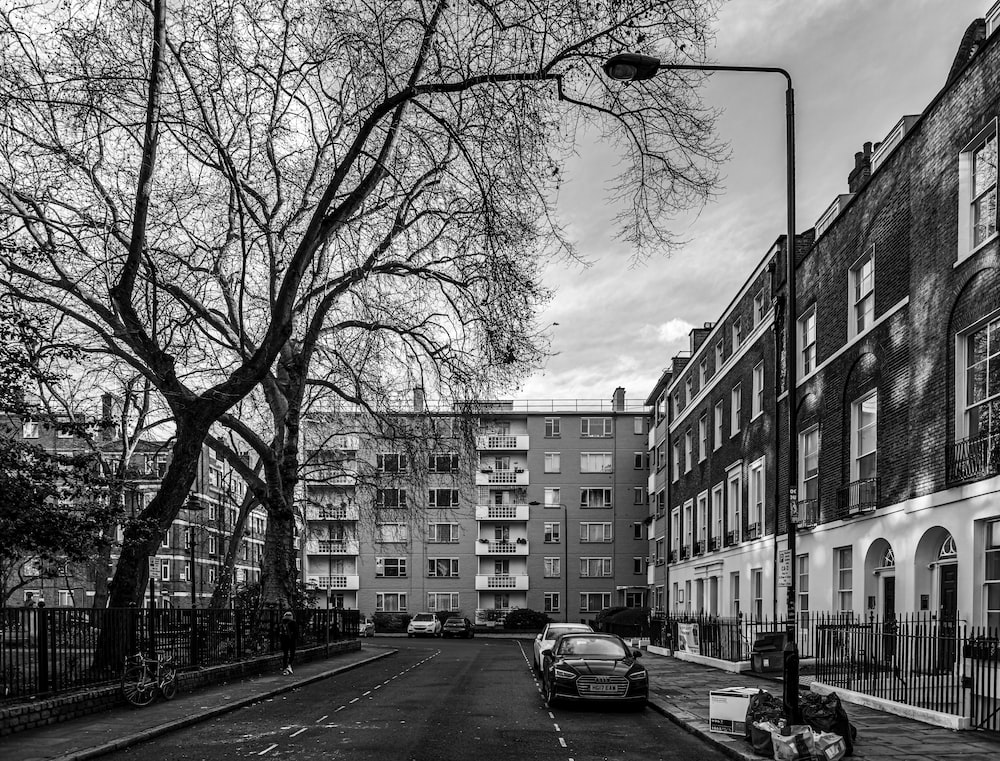
\includegraphics[width=6cm]{grayscale.jpeg}
\end{align*}

\begin{minted}[bgcolor=lightgray]{python}
    # The Code below takes in an image and converts into gray scaled if its coloured
    # Resizes it to 512*512
    # And at last it reads the image as an array and saves it 
    image = Image.open("grayscale.jpeg").convert("L")
    initial_size = image.size  # Store the initial size of the image
    desired_size = (512, 512)
    image = image.resize(desired_size, Image.ANTIALIAS)
    image_array = np.array(image)
    \end{minted}

The Updated Image below is resized to 512*512 \\
\begin{align*}
    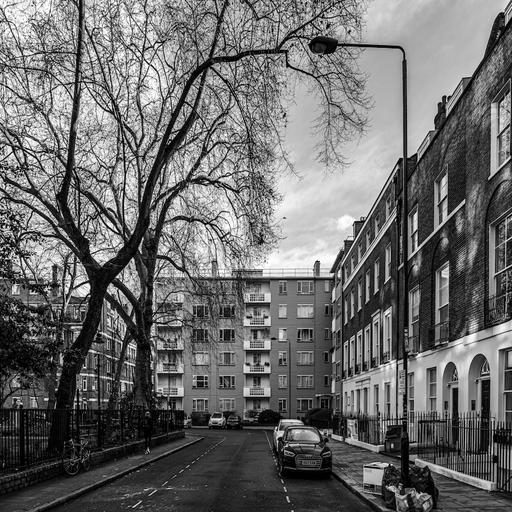
\includegraphics[width=6cm]{Image.jpeg}
\end{align*}
    
As we discussed, we are going to restrict ourselves to the 8x8 dimension. Therefore, we will work with the 512x512 image by splitting it into blocks of 8x8 images and working on them individually.
Now,We need to compute the Wavelet Transformtion of each 8x8 block
Since Wavelet Transformation can just be computed by multiplying with the Haar Transformation Matrix, we store the required matrices i.e., the Haar Transformation Matrix, The Transpose of Haar Transformation matrix and the their respective inverses

The code below indexes upon the 512x512 array and makes blocks of 8x8 and we compute the Haar Wavelet Matrix and as per the given input of threshold value we make changes in the Haar Wavlet Matrix and update them in the main image matrix
\begin{minted}[bgcolor=lightgray]{python}
    # The code below indexes upon the 512x512 array and makes blocks of 8x8 
    # We compute the Haar Wavelet Matrix 
    # It is easily computed using the stored values of Haar Transformation Matrices
    # As per the given input of threshold value we make changes in the Wavlet Matrix 
    # The Main image matrix is also updated at last
    H = np.array([[0.125, 0.125, 0.25, 0, 0.5, 0, 0, 0],
            [0.125, 0.125, 0.25, 0, -0.5, 0, 0, 0],
            [0.125, 0.125, -0.25, 0, 0, 0.5, 0, 0],
            [0.125, 0.125, -0.25, 0, 0, -0.5, 0, 0],
            [0.125, -0.125, 0, 0.25, 0, 0, 0.5, 0],
            [0.125, -0.125, 0, 0.25, 0, 0, -0.5, 0],
            [0.125, -0.125, 0, 0.25, 0.5, 0, 0, 0.5],
            [0.125, -0.125, 0, -0.25, 0, 0, 0, -0.5]])
    H_transpose = H.T
    H_transpose_inverse = np.linalg.inv(H_transpose)
    H_inverse = np.linalg.inv(H)
    Threshold_value = float(input("Enter the Threshold Value: "))
    block_size = 8

    # Compression
    compressed_image_array = np.copy(image_array)
    for i in range(0, image_array.shape[0], block_size):
        for j in range(0, image_array.shape[1], block_size):
            A = image_array[i:i+block_size, j:j+block_size]
            B_Matrix = np.dot(H_transpose, A)
            B = np.dot(B_Matrix, H)
            for k in range(8):
                for l in range(8):
                    if np.abs(B[k][l]) <= Threshold_value:
                        B[k][l] = 0
            final = np.dot(H_transpose_inverse, B)
            FinalA = np.dot(final, H_inverse)
            compressed_image_array[i:i+block_size, j:j+block_size] = FinalA
    #Atlast we save the compressed image
    compressed_image = Image.fromarray(compressed_image_array)
    reconstructed_image = compressed_image.resize(initial_size, Image.ANTIALIAS)
    # Reverting to original size
    reconstructed_image.save("RECONSTRUCTED.jpeg")
    \end{minted}
The following images show the variation of their quality with respect to the input threshold values.
\begin{figure}[htbp]
    \centering
    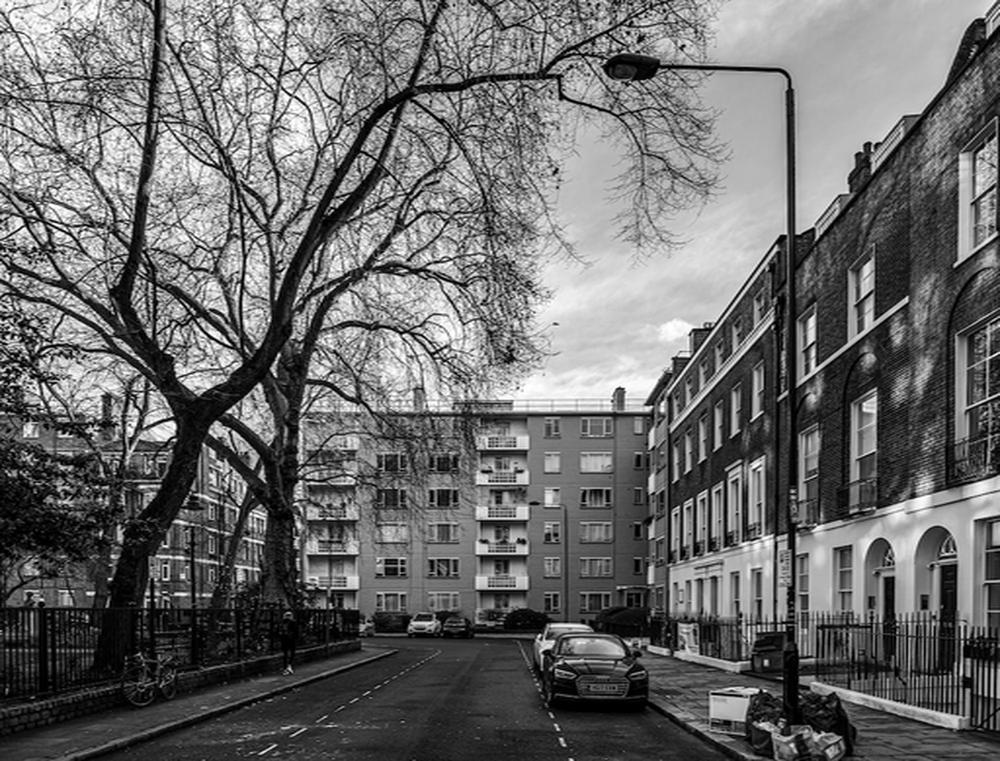
\includegraphics[width=6cm]{RECONSTRUCTED0.jpeg}
    \caption{Threshold: 0}
\end{figure}

The above image is exactly the same as the original image. This is because the threshold value is set to zero, perfectly depicting lossless compression.

\begin{figure}[htbp]
    \centering
    \begin{subfigure}{0.3\textwidth}
        \centering
        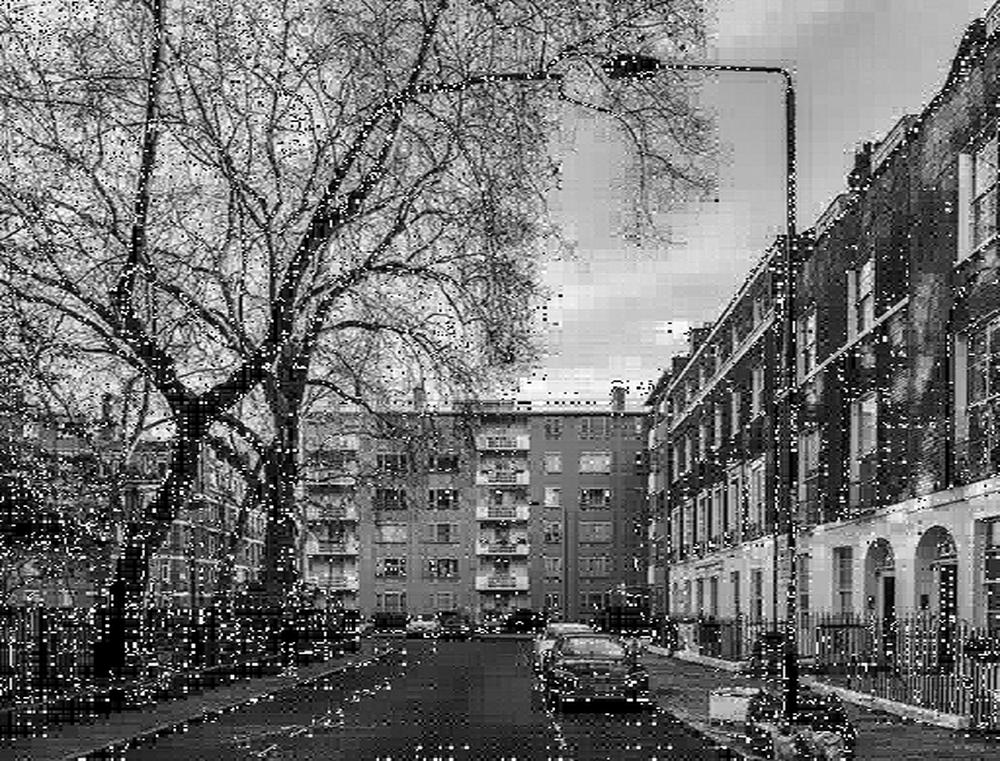
\includegraphics[width=\linewidth]{RECONSTRUCTED10.jpeg}
        \caption{Threshold: 10}
    \end{subfigure}\hfill
    \begin{subfigure}{0.3\textwidth}
        \centering
        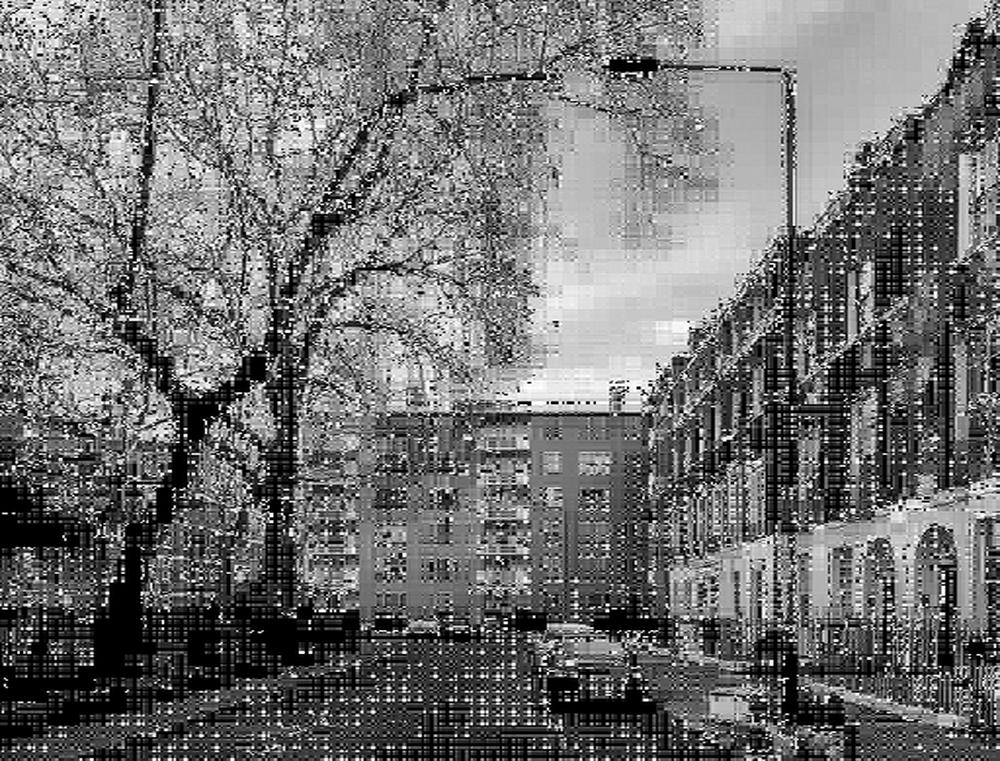
\includegraphics[width=\linewidth]{RECONSTRUCTED20.jpeg}
        \caption{Threshold: 20}
    \end{subfigure}\hfill
    \begin{subfigure}{0.3\textwidth}
        \centering
        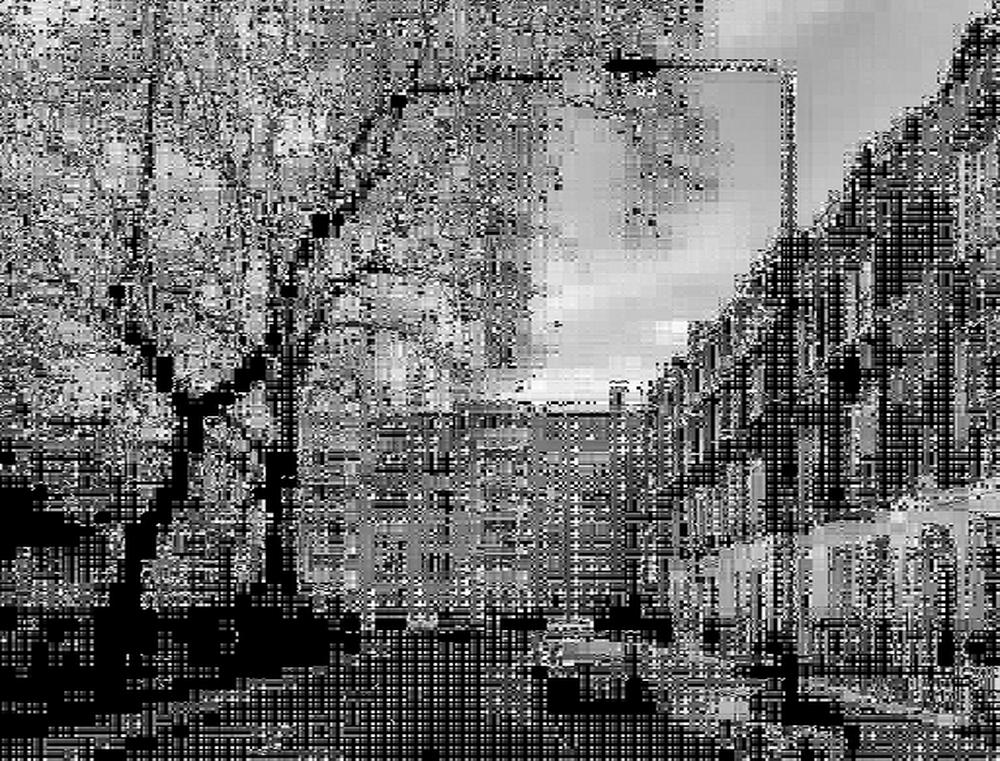
\includegraphics[width=\linewidth]{RECONSTRUCTED30.jpeg}
        \caption{Threshold: 30}
    \end{subfigure}

    \vspace{0.5cm}

    \begin{subfigure}{0.3\textwidth}
        \centering
        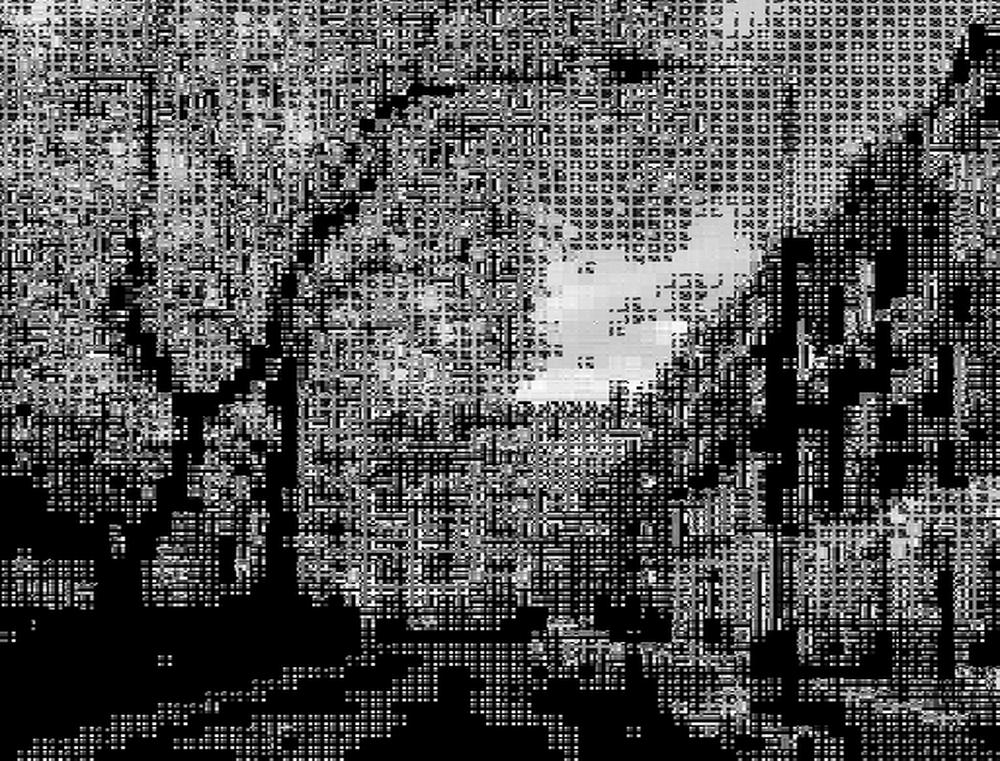
\includegraphics[width=\linewidth]{RECONSTRUCTED50.jpeg}
        \caption{Threshold: 50}
    \end{subfigure}\hfill
    \begin{subfigure}{0.3\textwidth}
        \centering
        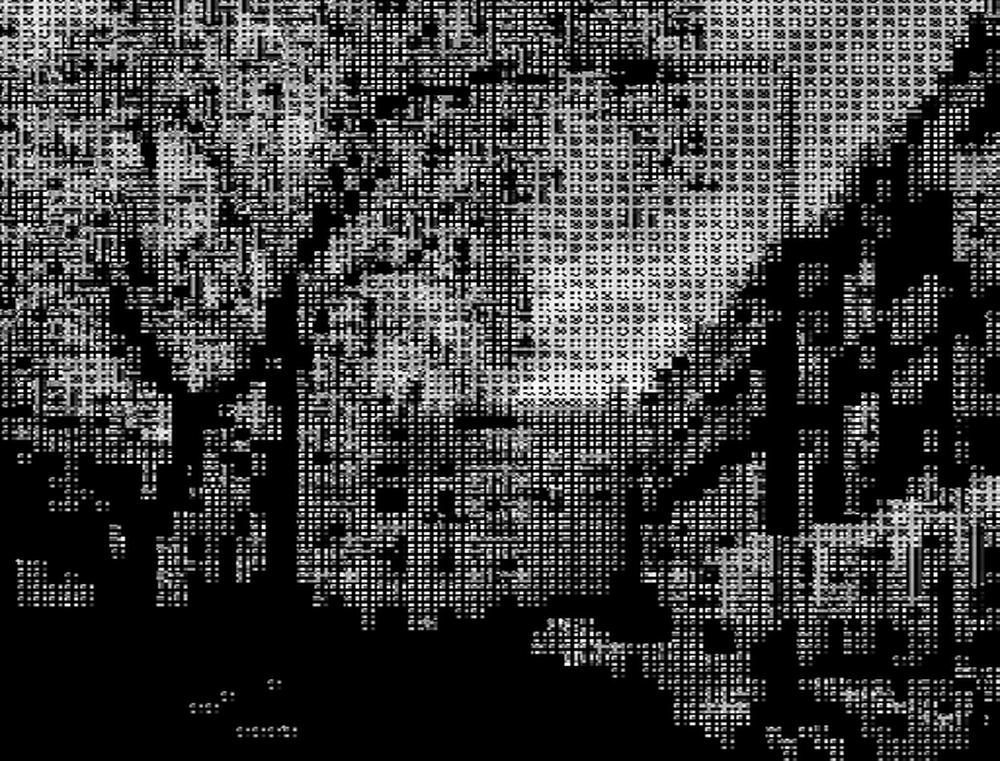
\includegraphics[width=\linewidth]{RECONSTRUCTED70.jpeg}
        \caption{Threshold: 70}
    \end{subfigure}\hfill
    \begin{subfigure}{0.3\textwidth}
        \centering
        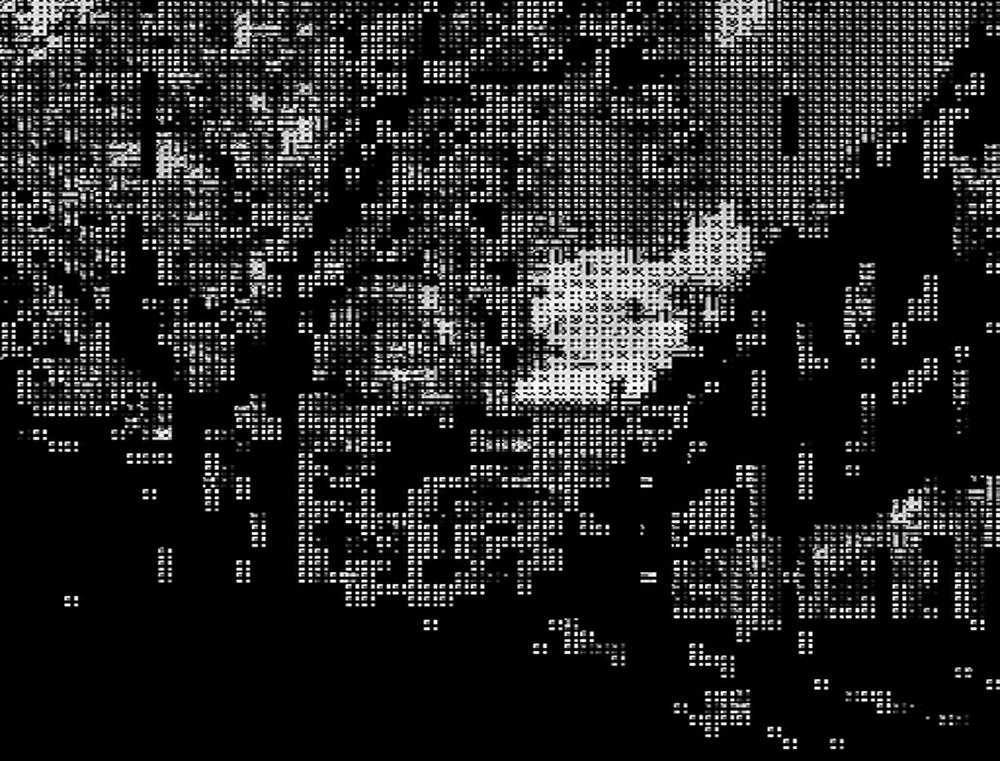
\includegraphics[width=\linewidth]{RECONSTRUCTED100.jpeg}
        \caption{Threshold: 100}
    \end{subfigure}

    \caption{Quality of Images decreases with increasing threshold value}
\end{figure}

A common question arises regarding the presence of white dots or artifacts in the compressed image after applying thresholding. These white dots are a consequence of the lossy nature of the compression process.

Hard thresholding is the technique that we have used to set coefficients below a certain threshold to zero. It is a simple and direct approach to reduce the size of the transformed coefficients and achieve compression. However, thresholding, particularly with hard thresholding, can lead to abrupt changes and introduce artifacts in the reconstructed image.

The opposite approach to hard thresholding is soft thresholding, where we decrease the value of transformed coefficients if they are found to be less than the threshold. This results in a smoother compression process and eliminates the presence of white dots.
\newpage

\subsection{Direct Cosine Transformation}

\setlength{\parindent}{1cm}
DCT stands for Discrete Cosine Transform, which is a mathematical technique used in signal and image processing to convert a signal or image from the spatial domain to the frequency domain. The DCT is closely related to the Discrete Wavelet Transform (DWT), as both are commonly employed in various applications such as data compression and feature extraction.
Both DCT and DWT involve changing the basis representation, removing high-frequency components, and reconstructing the image, the specific techniques and properties of the two transforms differ, leading to different compression characteristics and applications.

\setlength{\parindent}{1cm}
The DCT is primarily used in compression standards such as JPEG. It transforms an image from the spatial domain to the frequency domain. The main steps involved in DCT-based compression are as follows:
\begin{itemize}
    \item Divide the image into small, non-overlapping blocks.
    \item Apply the DCT to each block, which results in a frequency representation.
    \item Quantize the transformed coefficients by discarding less significant information.  
    \item During reconstruction, reverse the steps to reconstruct the image, applying an inverse DCT.
\end{itemize}

You can notice that the base algorithm of DCT is same as DWT they work in a similar way but, they differ greatly in the basic functions they use.The DCT uses only cosine functions as its basis functions, while the DWT employs a set of wavelet functions as its basis functions. The cosine basis functions used in DCT are symmetric and oscillate at a single frequency, whereas the wavelet basis functions used in DWT have different scales and can capture localized features at different resolutions.

Below are the basic functions that are used in DCT for one dimension:
    \begin{align*}
    X(k) &= \sqrt{\frac{2}{N}} \cdot C(k) \cdot \sum_{n=0}^{N-1} x(n) \cdot \cos\left(\frac{\pi}{N} \cdot (n + 0.5) \cdot k\right), \\
    &\text{for } k = 0 \text{ to } N-1,
    \end{align*}
and for 2-dimensional DCT is applied to image blocks, typically 8x8 or 16x16 pixels. The two-dimensional DCT is obtained by applying the one-dimensional DCT separately to each row and then to each column of the image block.
The formula for the two-dimensional DCT of an image block f(x, y) of size N x N is:
    \begin{align*}
    F(u, v) &= \sqrt{\frac{2}{N}} \cdot C(u) \cdot C(v) \cdot \sum_{x=0}^{N-1} \sum_{y=0}^{N-1} f(x, y) \cdot \cos\left(\frac{\pi}{N} \cdot (x + 0.5) \cdot u\right) \cdot \cos\left(\frac{\pi}{N} \cdot (y + 0.5) \cdot v\right), \\
    &\text{for } u, v = 0 \text{ to } N-1,
    \end{align*}
    where F(u, v) represents the transformed coefficients, C(u) and C(v) are the scaling factors, and (x, y) are the spatial coordinates of the image block.
    Similar to the one-dimensional DCT, F(0, 0) represents the DC component, and F(u, v) for u, v greater than 0 represents the AC components at different frequencies.
\end{document}

